%
% frequenzlokalisierung.tex -- slide template
%
% (c) 2021 Prof Dr Andreas Müller, OST Ostschweizer Fachhochschule
%
\bgroup

\def\kurve#1#2{
        \draw[color=#2,line width=1.4pt]
                plot[domain=0:6.3,samples=400]
                        ({\x},{7*\x*exp(-(\x/#1)*(\x/#1))/#1});
}
\definecolor{darkgreen}{rgb}{0,0.6,0}

\begin{frame}[t]
\setlength{\abovedisplayskip}{5pt}
\setlength{\belowdisplayskip}{5pt}
\frametitle{Lokalisierung}
\vspace{-20pt}
\begin{columns}[t,onlytextwidth]
\begin{column}{0.48\textwidth}
\begin{block}{Bandpass}
Gegeben durch $g(\lambda)\ge 0$:
\begin{align*}
g(0)                             &= 0\\
\lim_{\lambda\to\infty}g(\lambda)&= 0
\end{align*}
\vspace{-10pt}
\begin{enumerate}
\item<3-> Fourier-transformieren
\item<4-> Amplituden mit $g(\lambda)$ multiplizieren
\item<5-> Rücktransformieren
\end{enumerate}
\end{block}
\end{column}
\begin{column}{0.48\textwidth}
\uncover<6->{%
\begin{block}{Tiefpass}
Gegeben durch $h(\lambda)\ge0$:
\begin{align*}
h(0)                             &= 1\\
\lim_{\lambda\to\infty}h(\lambda)&= 0
\end{align*}
\vspace{-10pt}
\begin{enumerate}
\item<8-> Fourier-Transformation
\item<9-> Amplituden mit $h(\lambda)$ multiplizieren
\item<10-> Rücktransformation
\end{enumerate}
\end{block}}
\end{column}
\end{columns}
\begin{center}
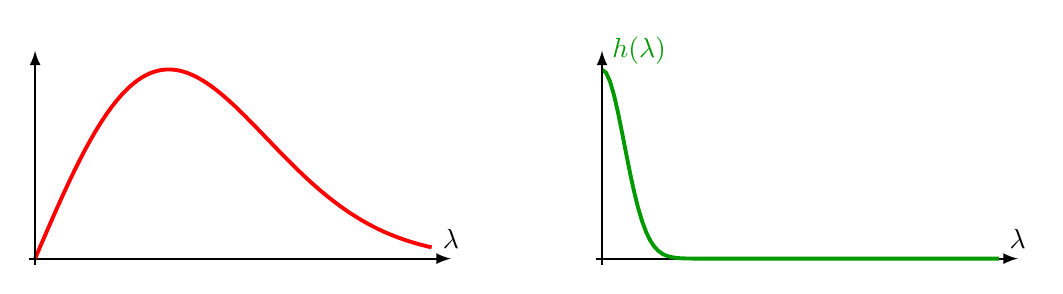
\begin{tikzpicture}[>=latex,thick,scale=0.8]

\uncover<2->{
\begin{scope}[xshift=-4.5cm]
\draw[->] (-0.1,0) -- (6.6,0) coordinate[label={$\lambda$}];
\kurve{3}{red}
\draw[->] (0,-0.1) -- (0,3.3);
\end{scope}
}

\uncover<7->{
\begin{scope}[xshift=4.5cm]
\draw[->] (-0.1,0) -- (6.6,0) coordinate[label={$\lambda$}];
\draw[color=darkgreen,line width=1.4pt]
        plot[domain=0:6.3,samples=100]
                ({\x},{3*exp(-(\x/0.5)*(\x/0.5)});

\draw[->] (0,-0.1) -- (0,3.3) coordinate[label={right:$\color{darkgreen}h(\lambda)$}];
\end{scope}
}

\end{tikzpicture}
\end{center}
\end{frame}
\egroup
